\documentclass[oneside,bibliography=totocnumbered,BCOR=5mm]{scrbook}

\usepackage[ngerman]{babel}

\usepackage{marvosym}
\usepackage{csquotes}

\usepackage[
backend=biber,
style=numeric,
citestyle=authoryear,
autocite=footnote
]{biblatex}
\addbibresource{bibliography.bib}
\addbibresource{extra.bib}

\usepackage{graphicx}
\graphicspath{ {images/} }

% \usepackage[hyphens]{url}
% \usepackage{hyperref}

\usepackage[sc]{mathpazo} % Use the Palatino font
\usepackage[T1]{fontenc} % Use 8-bit encoding that has 256 glyphs
\linespread{1.05} % Line spacing - Palatino needs more space between lines
\usepackage{microtype} % Slightly tweak font spacing for aesthetics

\usepackage[hmarginratio=1:1,top=32mm,columnsep=20pt]{geometry} % Document margins
\usepackage[hang, small,labelfont=bf,up,textfont=it,up]{caption} % Custom captions under/above floats in tables or figures
\usepackage{booktabs} % Horizontal rules in tables
\usepackage{lettrine} % The lettrine is the first enlarged letter at the beginning of the text
\usepackage{enumitem} % Customized lists
\setlist[itemize]{noitemsep} % Make itemize lists more compact

% \usepackage{abstract} % Allows abstract customization
% \renewcommand{\abstractnamefont}{\normalfont\bfseries} % Set the "Abstract" text to bold
% \renewcommand{\abstracttextfont}{\normalfont\small\itshape} % Set the abstract itself to small italic text

% \usepackage{titlesec} % Allows customization of titles
%\renewcommand\thesection{\Roman{section}} % Roman numerals for the sections
%\renewcommand\thesubsection{\roman{subsection}} % roman numerals for subsections
% \titleformat{\section}[block]{\large\scshape\centering}{\thesection.}{1em}{} % Change the look of the section titles
% \titleformat{\subsection}[block]{\large}{\thesubsection.}{1em}{} % Change the look of the section titles

\usepackage{fancyhdr} % Headers and footers
\pagestyle{fancy} % All pages have headers and footers
\fancyhead{} % Blank out the default header
\fancyfoot{} % Blank out the default footer
% \fancyhead[C]{Ethics in Progress (EiP) $\bullet$ 2019 } % Custom header text
% \fancyfoot[RO,LE]{\thepage} % Custom footer text

\usepackage{titling} % Customizing the title section

\usepackage{listings}
\usepackage{color}
\definecolor{mygreen}{rgb}{0,0.6,0}
\definecolor{mygray}{rgb}{0.5,0.5,0.5}
\definecolor{mymauve}{rgb}{0.58,0,0.82}

\lstset{
  backgroundcolor=\color{white},   % choose the background color; you must add \usepackage{color} or \usepackage{xcolor}; should come as last argument
  basicstyle=\footnotesize,        % the size of the fonts that are used for the code
  breakatwhitespace=false,         % sets if automatic breaks should only happen at whitespace
  breaklines=true,                 % sets automatic line breaking
  captionpos=b,                    % sets the caption-position to bottom
  commentstyle=\color{mygreen},    % comment style
  deletekeywords={...},            % if you want to delete keywords from the given language
  escapeinside={\%*}{*)},          % if you want to add LaTeX within your code
  extendedchars=true,              % lets you use non-ASCII characters; for 8-bits encodings only, does not work with UTF-8
  firstnumber=1,                % start line enumeration with line 1000
  frame=single,	                   % adds a frame around the code
  keepspaces=true,                 % keeps spaces in text, useful for keeping indentation of code (possibly needs columns=flexible)
  keywordstyle=\color{blue},       % keyword style
  language=Octave,                 % the language of the code
  morekeywords={*,...},            % if you want to add more keywords to the set
  numbers=left,                    % where to put the line-numbers; possible values are (none, left, right)
  numbersep=5pt,                   % how far the line-numbers are from the code
  numberstyle=\tiny\color{mygray}, % the style that is used for the line-numbers
  rulecolor=\color{black},         % if not set, the frame-color may be changed on line-breaks within not-black text (e.g. comments (green here))
  showspaces=false,                % show spaces everywhere adding particular underscores; it overrides 'showstringspaces'
  showstringspaces=false,          % underline spaces within strings only
  showtabs=false,                  % show tabs within strings adding particular underscores
  stepnumber=1,                    % the step between two line-numbers. If it's 1, each line will be numbered
  stringstyle=\color{mymauve},     % string literal style
  tabsize=2,	                   % sets default tabsize to 2 spaces
  title=\lstname                   % show the filename of files included with \lstinputlisting; also try caption instead of title
}

\definecolor{mygrey}{RGB}{28,28,28}
\newcommand{\codeinline}[1]{\colorbox{mygray}{\csname lstinline\endcsname!#1!}}

\begin{document}

% Titelseite
% \pagestyle{empty}       % keine Seitennummer
\begin{titlepage}
\begin{center}

\includegraphics{htw-logo.jpg}
\linebreak[4]
\linebreak[4]
\linebreak[4]
\linebreak[4]
\textit{\large Entwicklung und Evaluation von Methoden zur Absenkung der Nutzungsschwelle von Kommandozeilen-Interfaces}
\linebreak[4]
\linebreak[4]
\linebreak[4]
Abschlussarbeit
\linebreak[4]
\linebreak[4]
zur Erlangung des akademischen Grades:
\linebreak[4]
\linebreak[4]
\textbf{Bachelor of Science (B.Sc.)}
\linebreak[4]
\linebreak[4]
an der
\linebreak[4]
\linebreak[4]
Hochschule f\"ur Technik und Wirtschaft (HTW) Berlin
\linebreak[4]
Fachbereich 4: Informatik, Kommunikation und Wirtschaft
\linebreak[4]
Studiengang \textit{Angewandte Informatik}
\linebreak[4]
\linebreak[4]
\linebreak[4]
1. Gutachter: Titel akademischer Grad Vorname Nachname\linebreak[4]
2. Gutachter: B.Sc. Moritz Wachter\linebreak[4]
\linebreak[4]
\linebreak[4]
\linebreak[4]
\linebreak[4]
Eingereicht von Jonathan Neidel [573619]
\linebreak[4]
\linebreak[4]
\linebreak[4]
\linebreak[4]
Datum

\end{center}
\end{titlepage}
\newpage

\thispagestyle{empty}
\vspace*{2.2cm}
\noindent
{\Huge Danksagung}\\
\vspace*{1.6cm} \\

% Kopfzeilen (automatisch erzeugt)
%\pagestyle{headings}
[Text der Danksagung]

% Seite mit Abstracts
\newpage
\thispagestyle{empty}
\section*{Zusammenfassung}
[Text der Zusammenfassung]

\section*{Abstract}
[Summary of the thesis]


\clearpage
%Seite 1
\pagenumbering{roman}
%\setcounter{page}{1}

\tableofcontents
\listoffigures
\listoftables
\lstlistoflistings
.
\newpage

\pagenumbering{arabic}
% \setcounter{page}{1}   % setzt Seitenzaehlung auf 1

% \fbox{\parbox{\linewidth}{
% }}

% \\
% \linebreak[4]

% \footnote{Erg\"anzende Informationen k\"onnen Sie auch in eine Fu"snote auslagern. Hier wird die Fu"snote dazu genutzt, um Ihnen bei Interesse am Thema Zitation vertiefende Quellen (z.B. \autocite{balzert2011} oder \autocite{franck2013}) anzubieten.}

% \begin{table}
% \caption{\"Ubersicht: Untersuchte Steinl\"ause}
% \centering
% \begin{tabular}{llr}
% \toprule
% \multicolumn{2}{c}{Untersuchte Objekte mit Lokation des Habitats} \\
% \cmidrule(r){1-2}
% ID (nickname) & Ort & Gr\"o"se/L\"ange (in mm) \\
% \midrule
% 1 (Rosalinde) & Berlin, Mauerpark & $1.4$ \\
% 2 (Devil in disguise) & Brandenburg, BER-Airport & $2.8$ \\
% 3 (Hannes) & Berlin, Olympia-Stadion & $2.1$ \\
% 4 (Her Majesty) & Berlin, Humboldt-Forum & $2.0$ \\
% \bottomrule
% \end{tabular}
% \end{table}

% \begin{lstlisting}[caption={Ein Beispiel: Hello World (Scala)}]
% object HelloWorld {
%   def main(args: Array[String]): Unit = {
%     println("Hello, world!")
%   }
% }
% \end{lstlisting}

\chapter{Einleitung}
\section{Hintergrund der Arbeit}
% [Beschreibung des groben Kontextes der Arbeit; im Detail sollten Sie dies im Grundlagenteil darstellen]

Die Kommandozeile und darauf basierende Applikationen bergen das Potential für Produktivitätssteigerungen im Vergleich zu GUI Applikationen, vorrausgesetzt der Nutzer weiß mit dieser umzugehen. % TODO: Citation needed


\section{Problem- und Zielstellung (Scope)}
% [Beschreibung der Problemstellung sowie der sich daraus ergebenden Teilprobleme,-ziele und Forschungsfrage(n), welche Sie mit Ihrer Arbeit addressieren]

Die Kommandozeile und seine Applikationen sind für Personen welche mit dieser Umgebung nicht vertraut sind schwer benutzbar. % TODO: Citation needed
Einflussfaktoren dafür sind:

\begin{enumerate}
  \item Fehlendes Wissen über das Ökosystem (wie werden Applikationen gestartet, wie findet man Hilfe, Verständnis grundsätzlicher Werkzeuge fehlt)
  \item Applikationen sind nicht für Neulinge konzipiert
\end{enumerate}

Problemstellung dieser Arbeit soll das zweite der gelisteten Probleme sein: Das Zusammentragen und Evaluieren der Faktoren welche Kommandozeilen Applikation für Neulinge zugänglich machen. Oder konkreter als Forschungsfrage definiert:

\bigbreak

\fbox{\parbox{\linewidth}{
Welche Faktoren sind für die Konstruktion einer Command-Line basierten App zu
beachten um diese für Personen, welche nicht mit dem Terminal vertraut sind,
zugänglich zu machen?
}}

\section{Aufbau der Arbeit}
% [Beschreibung des Aufbaus der Arbeit]

Die Arbeit gliedert sich in folgende drei Hauptteile:

\begin{enumerate}
  \item \textbf{Erarbeitung von Methoden zur Absenkung der Nutzungsschwelle von Kommandozeilen Interfaces}:
    \smallbreak
    In Literaturrecherche werden Methoden zusammengetragen und formuliert.
    Diese sind - wie im Sinne des Wortes Methode (``Weg zu etwas hin'' laut \cite{duden_methode}) - deskriptiv und beschreiben wie ein gewünschter Effekt zu erzielen sein soll.
    \begin{enumerate}
      \item \textbf{Probleme mit Kommandozeilen Interfaces}:
        \smallbreak
        Es werden zuerst Probleme, welche die Nutzung von Kommandozeilen Interfaces erschweren erläutert.
      \item \textbf{Methoden zur Absenkung der Nutzungsschwelle von Kommandozeilen Interfaces}:
        \smallbreak
        Methoden werden formuliert und wie diese zuvor geschilderte Probleme adressieren.
    \end{enumerate}

  \item \textbf{Implementation einer Anwendung auf Basis der erarbeiteten Methoden}:
    \smallbreak
    Gesammelte Methoden werden in der Implementation einer App demonstriert.
    Die App ist überschaubar komplex und adressiert das manuelle Festhalten von Arbeitsstunden.
    \begin{enumerate}
      \item \textbf{Anforderungsanalyse}:
        \smallbreak
        Zuerst werden die von der App zu erfüllenden Anforderungen erörtert.
      \item \textbf{Implementation der App unter Berücksichtigung gesammelter Methoden}:
        \smallbreak
        Es werden die Anforderungen unter Beachtung ermittelter Methoden implementiert.
    \end{enumerate}

  \item \textbf{Evaluation der implementierten Anwendung}:
    \smallbreak
    Die App wird von mit dem Anwendungsfall vertrauten Kommandozeilen Einsteigern getestet.
    Und Anhand einer Umfrage evaluiert.
    \begin{enumerate}
      \item \textbf{Umfragengestaltung}:
        \smallbreak
        Es wird die Umfrage gestaltet.
      \item \textbf{Auswertung}:
        \smallbreak
        Ergebnisse der Umfrage werden ausgewertet.
    \end{enumerate}
\end{enumerate}

\chapter{Grundlagen und Definitionen}
% [Beschreibung des Kontextes der Arbeit mit allen durch die Problemstellung tangierten Bereichen, Methoden, Theorien, Erkenntnissen, Technologien, ... ]

% TODO: CLI, how did we get here, <-> GUI

% TODO: citation needed, multiple tech definitions
\textbf{Kommandozeilen Interface}: (Engl. command-line interface) oft auch als \textbf{CLI} abgekürzt

Die Kommandozeile nimmt eine Anfrage, in Form von einer Zeile Text, entgegen und antwortet darauf.

\begin{figure}
  \centering
  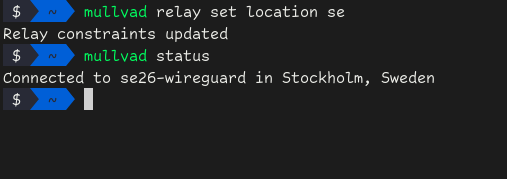
\includegraphics[scale=0.5]{mullvad-status.png}
  \caption{Ändern und Überprüfen des VPN Standorts in der Linux Kommandozeile mit dem \codeinline{mullvad} CLI}
  \label{fig:mullvad-status}
\end{figure}

Die Kommandozeile existiert in zwei Ausprägungen: dem Betriebssystem CLI, auch als Shell bekannt (siehe die Linux Shell in Abbildung \ref{fig:mullvad-status}) oder der Kommandozeile einer Anwendung (siehe die Node.js Kommandozeile in Abbildung \ref{fig:node-calc}).

\begin{figure}
  \centering
  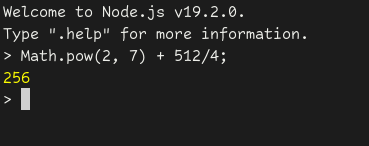
\includegraphics[scale=0.5]{node-calc.png}
  \caption{Durchführung einer Berechnung in der Node.js Kommandozeile}
  \label{fig:node-calc}
\end{figure}

\cite{Spolsky_2001} beschreibt neben der CLI noch zwei weitere Terminal Interfaces welche sich aus diesem entstanden sind:
\\
\textbf{Interaktive CLI}: Ein ``question and answer model'' \parencite[42]{Spolsky_2001} der Kommandozeile, wo der Nutzer mittels Fragen, auf die eine Antwort erwartet wird, entlastet wird. Mehr dazu in Kapitel \ref{chap:interactive}.
\\
\textbf{Menu-driven CLI}: auch als Ncurses CLI bekannt. Das Menü-basierte CLI ähnelt dem GUI indem

% Vergleich zu GUI
% function-orient vs object-oriented vgl. nielson1993

%%% Methoden
\chapter{Methoden zur Absenkung der Nutzungsschwelle von Kommandozeilen Interfaces}
% TODO: intro here

\section{Methodologie}
% [Beschreibung des geplanten Vorgehens(-modells) zur Lösung der Problemstellung; umfasst u.a.:

Die Artefakte dieses Kapitels sind die folgenden:
\begin{enumerate}
  \item Eine Auflistung von Problemen welche den Umgang mit Kommandozeilen Interfaces erschweren
  \item Eine Auflistung von Methoden, welche diese Probleme adressieren
\end{enumerate}

In Literaturrecherche sollen Probleme erschlossen werden, als auch die dafür -
möglicherweise vielfach - vorliegenden Lösungsansätze. Welche dann, unter Bezug
auf das Problem, als Methoden formuliert dokumentiert werden sollen.
\\
Die Formulierung als Methode soll dabei den Lösungsansatz so beschreiben das
dieser anwendbar ist. Dies ist u.a. erforderlich da die Methoden im nächsten
Schritt angewandt werden sollen.

\section{Probleme mit Kommandozeilen Interfaces}

Es folgen, in nicht priorisierter Reihenfolge, Probleme welche die
Nutzungsschwelle von Kommandozeilen Interfaces erhöhen, d.h. diese weniger
zugänglich.
\\
Diese bestmöglich zu adressieren sollte zu einer Absenkung der Nutzungsschwelle
und damit besser zugänglichen Applikationen führen.

\subsection{Erinnern von Kommandos}

Ein Hauptproblem stellt sich darin das der Nutzer alle - für den Anwendungsfall
relevanten - Kommandos und Parameter wissen muss um die Schnittstelle nutzen zu
können \parencite{Raskin_2008}.

\begin{figure}
  \centering
  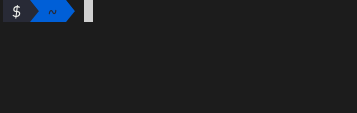
\includegraphics[scale=0.5]{empty-prompt.png}
  \caption{Ohne Wissen um Kommandos passiert nichts}
\end{figure}


\section{Gesammelte Methoden}

\subsection{Interaktive CLI}
\label{chap:interactive}

% Methoden beziehen sich direkt auf ein Problem welches adressiert werden soll.

%%% Bauen
\chapter{Anforderungsanalyse}
% [Beschreibung der Erhebung, Granularisierung und Priorisierung der zu Grunde liegenden Anforderungen]
\section{Konzept}
\section{Anforderungen}
% Anforderungserhebung nur durch mich, da App nicht Fokus der Arbeit und ich User bin

\chapter{Implementation der App unter Berücksichtigung gesammelter Methoden}
\section{Fundament}

Das Fundament der App stellen die zugrundelegenden technologischen Aspekte dar,
welche nicht oder nur indirekt die Nutzbarkeit, und damit den Fokus der Arbeit
betreffen.
% ... get into tech

\section{Anwendung gesammelter Methoden}
% hier List wie die Methoden angewandt wurden

%%% Umfrage
\chapter{Umfragengestaltung}
\section{Methodologie}
\section{Ergebnisartefakte}
% [Beschreibung der Ergebnisse / Ergebnistypen, welche Sie im Rahmen der Probleml\"osung generieren / erzielen wollen, z.B. Algorithmus, Prototyp einer Software(komponente), ... ]

\chapter{Auswertung}

%%% Finish
\chapter{Zusammenfassung}
% [Aggregierte retrograde Kurzbeschreibung der Arbeit]
\section{Schlussfolgerungen}
% [Beschreibung der insgesamt zu konstatierenden Schlussfolgerungen im Zusammenhang mit der Arbeit]
\section{Limitationen}
% [Beschreibung der Ergebnisse einer kritischen Reflektion und Begr\"undung dessen, was die Arbeit nicht zu leisten vermag]
\section{Ausblick}
% [Beschreibung und Begr\"undung potenzieller zuk\"unftiger Folgeaktivit\"aten im Zusammenhang mit Ihrer Arbeit (z.B. weitere Anforderungen, Theoriebildung, ... ]

%%% possible modules
% \section{Kontext}
% \subsection{Domain}
% \subsection{Technologien}
% \subsection{Methoden und Konzepte}
% \section{...}
% \subsection{...}
% \subsection{...}
% \chapter{Anforderungserhebung und -analyse}
% \section{Nutzer- und Systemanforderungen}
% \subsection{Funktionale Anforderungen}
% \subsubsection{Obligatorisch (MUSS)}
% \subsubsection{Fakultativ (Kann)}
% \subsection{Nicht-funktionale Anforderungen}
% \subsubsection{Obligatorisch (MUSS)}
% \subsubsection{Fakultativ (Kann)}
% \section{...}
% \chapter{Konzeption \& Entwurf}
% [Beschreibung des Entwurfs auf Basis der Methodologie / der geplanten Vorgehensweise zur Probleml\"osung im Kontext der Anforderungen (i.A. der Art der Arbeit)]
% \section{Prozess}
% \section{Systemarchitektur}
% \section{Softwarearchitektur}
% \section{Schnittstellen}
% \section{Datenmanagement}
% \section{...}
% \chapter{Implementierung}
% [Beschreibung der Implementierung\footnotemark auf Basis des Entwurfs und der Methodologie / der geplanten Vorgehensweise zur Probleml\"osung im Kontext der Anforderungen. Hier ist Raum f\"ur Listings, wie z.B. das nun Folgende: Umfangreicher Quell-Code sollte in den Anhang ausgelagert werden.]
% \chapter{Test}
% [Beschreibung, wie Sie auf Basis des geplanten Testvorgehens was mit welchen Kriterien und Technologien getestet haben]
% \chapter{Darstellung und Bewertung der Ergebnisse}
% [Beschreibung der Ergebnisse aus allen voran gegangenen Kapiteln sowie der zuvor generierten Ergebnisartefakte mit Bewertung, wie diese einzuordnen sind]

% \bibliographystyle{apalike}
% \bibliographystyle{ksfh_nat} % ein anderer Stil
% \bibliography{science}
\printbibliography[
heading=bibintoc,
title={Quellenverzeichnis}
]

\newpage

\chapter{Abk\"urzungsverzeichnis}
\newpage
\chapter{Glossar}
\begin{appendix}
\pagenumbering{Roman}
\chapter{Appendix}

\section{Quell-Code}

\section{Tipps zum Schreiben Ihrer Abschlussarbeit}

\begin{itemize}
\item Achten Sie auf eine neutrale, fachliche Sprache. Keine \glqq{}Ich\grqq{}-Form.
\item Zitieren Sie zitierf\"ahige und -w\"urdige Quellen (z.B. wissenschaftliche Artikel und Fachb\"ucher; nach M\"oglichkeit keine Blogs und keinesfalls Wikipedia.
\item Zitieren Sie korrekt und homogen.
\item Verwenden Sie keine Fu{\ss}noten f\"ur die Literaturangaben.
\item Recherchieren Sie ausf\"uhrlich den Stand der Wissenschaft und Technik.
\item Achten Sie auf die Qualit\"at der Ausarbeitung (z.B. auf Rechtschreibung).
\item Informieren Sie sich ggf. vorab dar\"uber, wie man wissenschaftlich arbeitet bzw. schreibt:
\begin{itemize}
\item Mittels Fachliteratur\footnote{Z.B. \autocite{balzert2011}, \autocite{franck2013}}, oder
\item Beim Lernzentrum\footnote{Weitere Informationen zum Schreibcoaching finden sich hier: \url{https://www.htw-berlin.de/studium/lernzentrum/studierende/schreibcoaching/}; letzter Zugriff: 13 VI 19.}.
\end{itemize}
\end{itemize}

\newpage
\thispagestyle{empty}
\noindent

\section*{Eidesstattliche Versicherung}
Hiermit versichere ich an Eides statt durch meine Unterschrift, dass ich die vorstehende Arbeit selbstst\"andig und ohne fremde Hilfe angefertigt und alle Stellen, die ich w\"ortlich oder ann\"ahernd w\"ortlich aus Ver\"offentlichungen entnommen habe, als solche kenntlich gemacht habe, mich auch keiner anderen als der angegebenen Literatur oder sonstiger Hilfsmittel bedient habe. Die Arbeit hat in dieser oder \"ahnlicher Form noch keiner anderen Pr\"ufungsbeh\"orde vorgelegen.\\
\linebreak[4]
\linebreak[4]
\linebreak[4]
\linebreak[4]
-------------------------------------------------------\linebreak[4]
Datum, Ort, Unterschrift

\end{appendix}
\end{document}
